%%
% This is an Overleaf template for presentations
% using the TUM Corporate Desing https://www.tum.de/cd
%
% For further details on how to use the template, take a look at our
% GitLab repository and browse through our test documents
% https://gitlab.lrz.de/latex4ei/tum-templates.
%
% The tumbeamer class is based on the beamer class.
% If you need further customization please consult the beamer class guide
% https://ctan.org/pkg/beamer.
% Additional class options are passed down to the base class.
%
% If you encounter any bugs or undesired behaviour, please raise an issue
% in our GitLab repository
% https://gitlab.lrz.de/latex4ei/tum-templates/issues
% and provide a description and minimal working example of your problem.
%%

\documentclass{setbeamer}

\usepackage{scrextend}
\changefontsizes{8pt}


\usepackage{tikz}
\usepackage{marvosym}
\usetikzlibrary{positioning,graphs,trees,matrix}
\usetikzlibrary{overlay-beamer-styles} % adds [visible on] option for tikz nodes
\usetikzlibrary{arrows.meta} % allows for more specification on how arrows look

\tikzset{
    >=Stealth[round],
    commit/.style = {draw, circle, minimum size = 7mm},
}

\newenvironment{mydirtree}[1][]{
    \begin{tikzpicture}[
        grow via three points = {one child at (0.3,-0.7) and two children at (0.3,-0.7) and (0.3,-1.3)},
        edge from parent path = {(\tikzparentnode.south) circle |- (\tikzchildnode.west)},
        every node/.style = {anchor=west},
        #1
    ]
}{
    \end{tikzpicture}
}


\TUMbeamersetup{
    section page = TUM toc,   % style of section pages
}

% presentation metadata
\title{Software Testing and Continuous Integration}
\subtitle{Concept and Usage}

\institute{\theChairName\\\theDepartmentName\\\theUniversityName}
\date[\today]{\today}

\footline{\insertauthor~|~\insertshorttitle~|~\insertshortdate}

\begin{document}

\maketitle

\section{Automated Software Testing}

\begin{frame}{Software Testing}{Motivation}
    \begin{enumerate}
        \item Software testing is the act of checking whether software satisfies expectations.
        \item Software testing can determine the correctness of software for specific scenarios, 	but cannot determine correctness for all scenarios.
        \item The practice of writing code to test the code,
and then run those tests in an automated fashion is called \textbf{Automated Software Testing}.
		\item Software testing should follow a ``pyramid'' approach wherein most of the tests are unit tests, followed by integration tests and finally end to end (e2e) tests.
    \end{enumerate}
    
\end{frame}

\begin{frame}{Testing Pyramid}

\vspace{1cm}

	\centering
    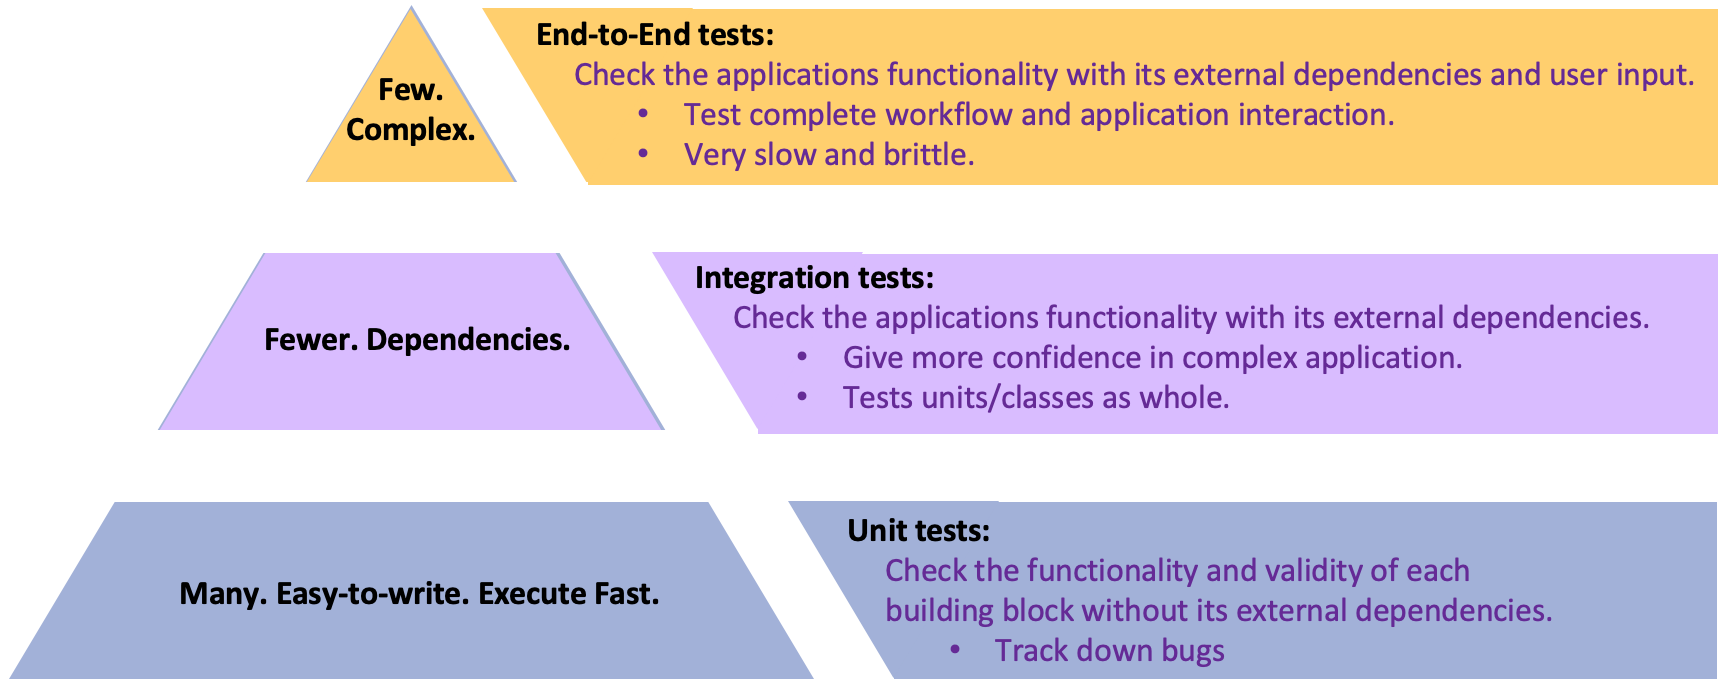
\includegraphics[width=12cm]{resources/test_pyramid.png}
    
\end{frame}


\begin{frame}{Software Testing Philosophies}

\vspace{1cm}

	\begin{columns}[T]
        \begin{column}{0.5\textwidth}
            \textbf{Adding Tests}\\
            \begin{itemize}
            	\item 
            	Add tests to check correctness of software.
            	\item
            	How many software tests? Application dependent...
            \end{itemize}
        \end{column}
        \begin{column}{0.5\textwidth}
            \textbf{Test-driven development}\\
            First write test, then code
            \begin{itemize}
            	\item 
            	Add a test for all functionality needed;
            	\item
            	Run all tests. The new test should fail for expected reasons;
            	\item
            	Write the simplest code that passes the new test;
            	\item 
            	Continue until tests pass;
            	\item
            	Refactor as needed, while preserving functionality;
            \end{itemize}
        \end{column}
	\end{columns}
        
    
\end{frame}

\begin{frame}{Software Testing Frameworks}
\vspace{.3cm}
Testing Frameworks provide easy software testing.
\begin{itemize}
\item Googletest is a popular ecosystem for testing C++ code \url{https://github.com/google/googletest}
\item pytest is a popular ecosystem for testing python code \url{https://docs.pytest.org/en/stable/}
\item Mocha is a popular ecosystem for testing Java code \url{https://github.com/mochajs/mocha}
\end{itemize}
\begin{columns}
\begin{column}{0.5\textwidth}
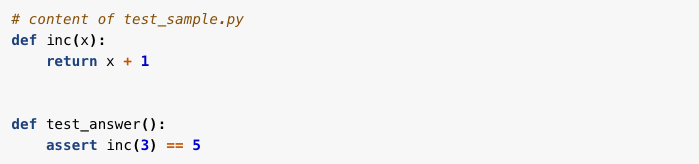
\includegraphics[width=7cm]{resources/pytest1.png}
\end{column}
\begin{column}{0.5\textwidth}
\vspace{1cm}
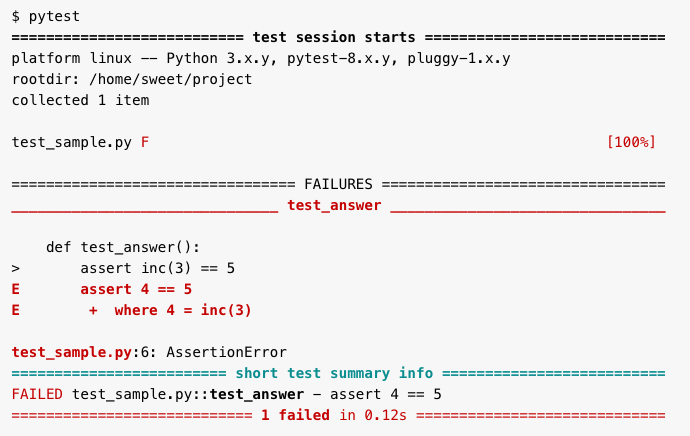
\includegraphics[width=7cm]{resources/pytest2.png} 
\end{column}
\end{columns}
  
      
\end{frame}


\begin{frame}[fragile]{pytest Hands-On}
    \begin{columns}
        \begin{column}{0.6\textwidth}
            \begin{TUMCodeBlock}{src/my$\_$math.py}{python}
def add_numbers(f1, f2):
	return f1 + f2
def subtract_numbers(f1, f2):
	return f1 - f2
def multiply_numbers(f1, f2):
	return f1 * f2
            \end{TUMCodeBlock}

            \begin{TUMCodeBlock}{src/example.py}{python}
from my_math import *

print("* Addition:")
print(" If I add 5 and 8, I get " + str(add_numbers(5, 8)) + ".")
print("* Subtraction:")
print(" If I subtract 5 from 8, I get " + str(subtract_numbers(8, 5)) + ".")
            \end{TUMCodeBlock}
        \end{column}
        \begin{column}{0.4\textwidth}

        \end{column}
    \end{columns}
\end{frame}


\begin{frame}[fragile]{pytest Hands-On}
    \begin{columns}
        \begin{column}{0.6\textwidth}
            \begin{TUMCodeBlock}{src/my$\_$math.py}{python}
def add_numbers(f1, f2):
	return f1 + f2
def subtract_numbers(f1, f2):
	return f1 - f2
def multiply_numbers(f1, f2):
	return f1 * f2
            \end{TUMCodeBlock}

            \begin{TUMCodeBlock}{src/example.py}{python}
from my_math import *

print("* Addition:")
print(" If I add 5 and 8, I get " + str(add_numbers(5, 8)) + ".")
print("* Subtraction:")
print(" If I subtract 5 from 8, I get " + str(subtract_numbers(8, 5)) + ".")
            \end{TUMCodeBlock}
        \end{column}
        \begin{column}{0.4\textwidth}
            \begin{TUMCodeBlock}{test/test$\_$example$\_$add.py}{python}
from src.my_math import add_numbers


def test_add_numbers():
    result = add_numbers(1, 2)
    assert result == 3
            \end{TUMCodeBlock}
            \begin{TUMCodeBlock}{test/test$\_$example$\_$subtract.py}{python}
from src.my_math import subtract_numbers


def test_subtract_numbers():
    result = subtract_numbers(1, 2)
    assert result == -1
            \end{TUMCodeBlock}
        \end{column}
    \end{columns}
\end{frame}




\begin{frame}[fragile]{pytest Hands-On}
    \begin{columns}
        \begin{column}{0.2\textwidth}
            \begin{TUMCodeBlock}{pytest.ini}{python}
[pytest]
pythonpath = .
            \end{TUMCodeBlock}
        \end{column}
        \begin{column}{0.6\textwidth}
        \vspace{1cm}
            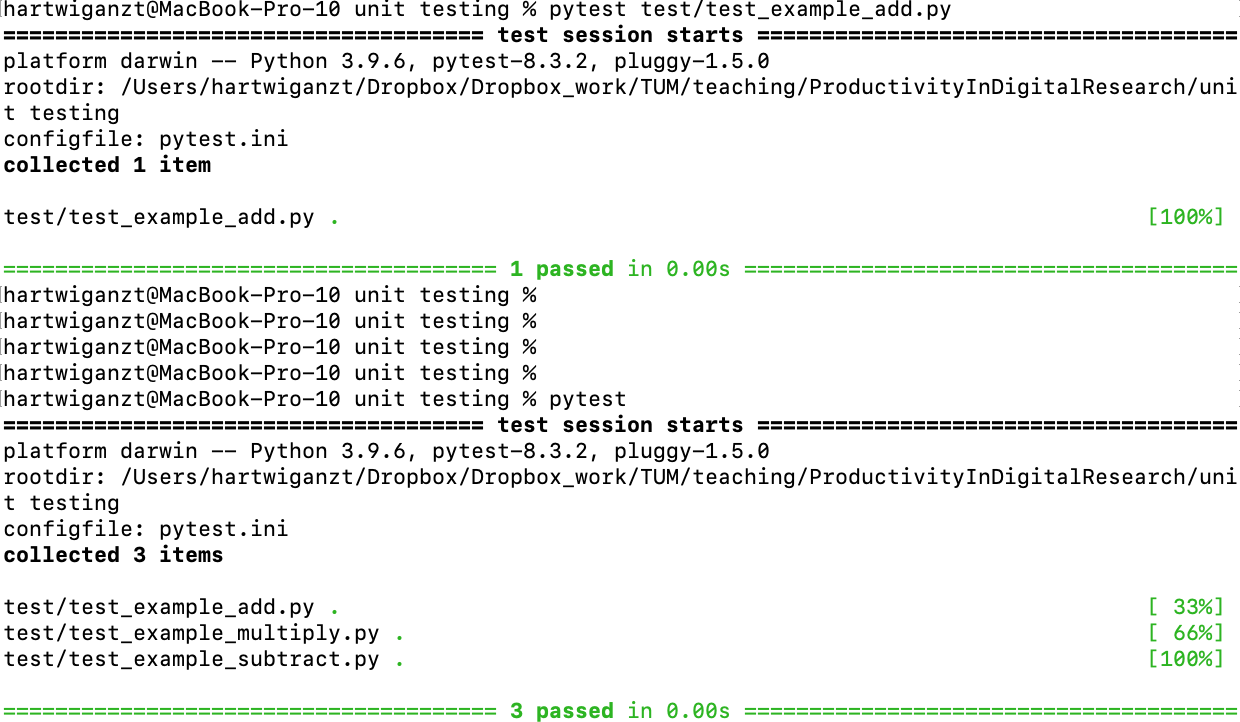
\includegraphics[width=\columnwidth]{resources/pytestmath}
        \end{column}
    \end{columns}


\end{frame}




\section{Continuous Integration}

\begin{frame}{Continuous Integration}{Motivation}
    \begin{enumerate}
        \item In code development, it is interesting to see whether any change breaks the compilation or execution of the code.
        \item Manually checking is very cumbersome.
        \item For popular code, checking a variety of operating systems, compilers, etc. is important.
        \item Best scenario: check after every change in the software repository.
    \end{enumerate}

\vspace{1cm}

Continuous Integration (CI) is an ``automated user'' that clones a repository, compiles and tests the code using a pre-defined command sequence in a pre-defined environment.   
    
\end{frame}



\begin{frame}[c]{CI Infrastructure}
    \begin{columns}[T]
        \begin{column}{0.5\textwidth}
            \textbf{Hardware}\\
            \begin{itemize}
            \item 
            A server is needed to clone the repository and compile the software.
            \item
            Git hosting sites offer CI as a service (GitHub actions, GitLab runners).
            \item 
            One can also host the CI on a local machine.
            \item 
            Some CI workflows require a variety of hardware architectures (x86, ARM, GPUs\dots)
            \end{itemize}
        \end{column}

        \begin{column}{0.5\textwidth}
            \textbf{Software}\\
            \begin{itemize}
            \item 
            The operating system and compiler/library environment can be configured.
            \item
            Often, containers (Docker, Singularity\dots) are used to package the environments.
            \item 
            CI can rely on several containers for testing different software environments.
            \end{itemize}
        \end{column}
    \end{columns}
\end{frame}

\begin{frame}[c]{CI with GitLab}
	\centering
    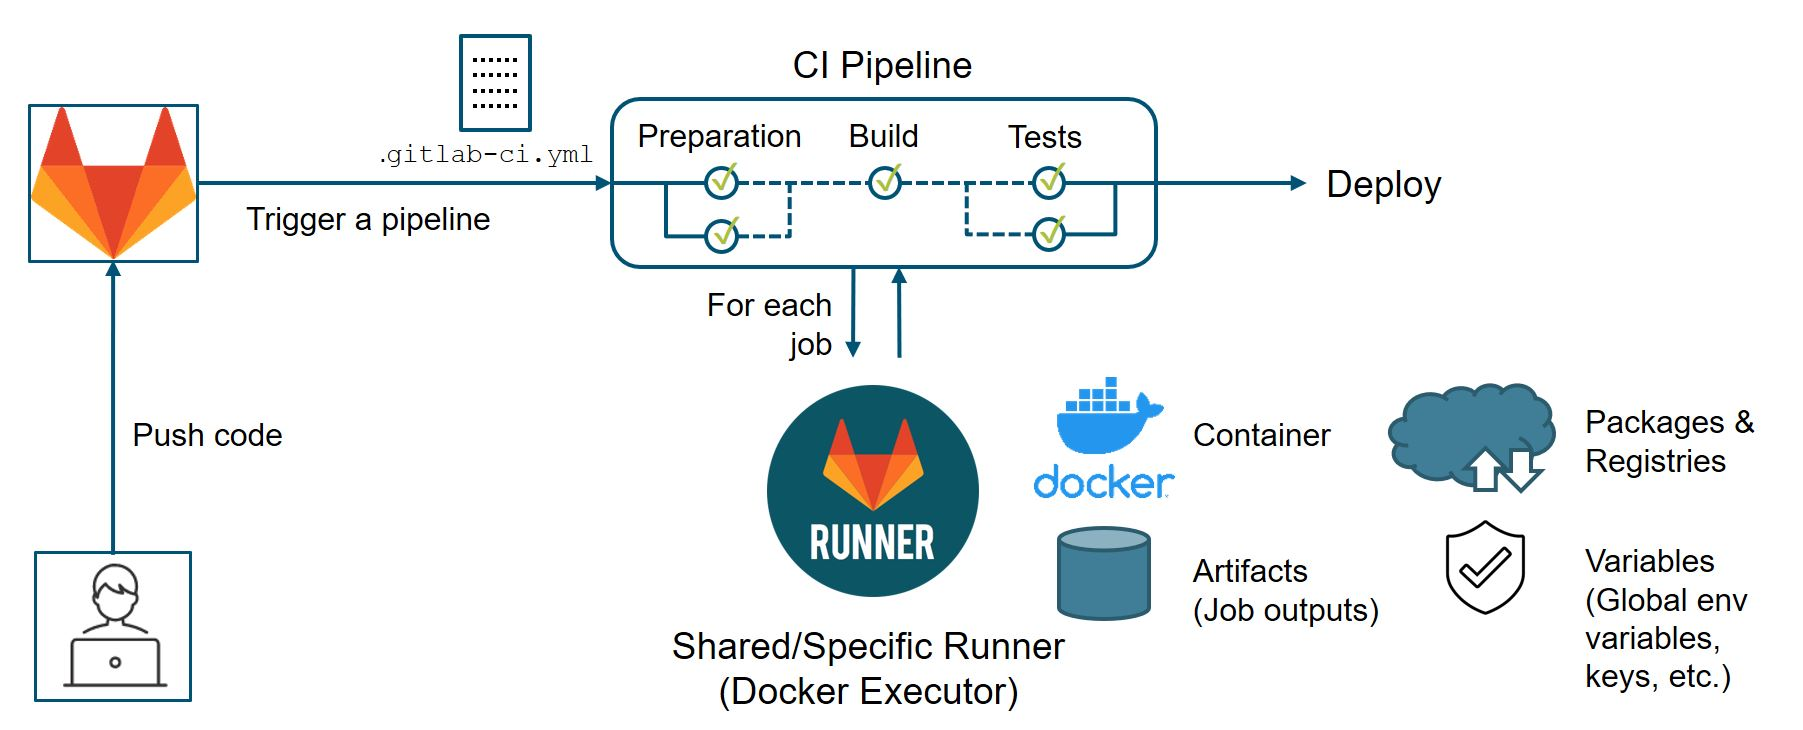
\includegraphics[width=15cm]{resources/ci-gitlab}
\end{frame}


\begin{frame}[fragile]{Configuring CI}
			\textbf{.gitlab-ci.yml} configures the CI instance and collects the commands forming a \textbf{CI pipeline}.

	% \centering
    %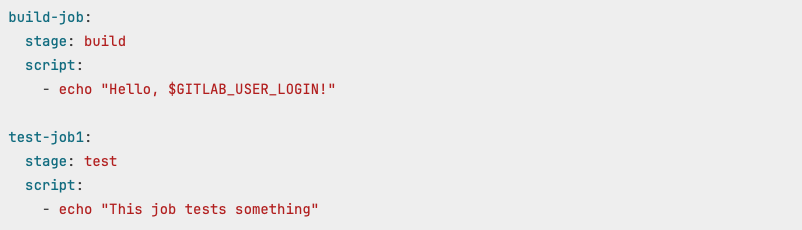
\includegraphics[width=10cm]{resources/ciyaml2.png}
\begin{TUMCodeBlock}{.gitlab-ci.yml}{markdown}
# image of an OS
image: ubuntu:20.04

pytest:
  stage: test
  before_script:
    # update ubuntu
    - apt-get update
    # install pip
    - apt-get install -y python3-pip
    # install python packages
    - pip3 install pytest
  script:
    # run pytest
    - pytest
\end{TUMCodeBlock}
            
            
\end{frame}

\begin{frame}[fragile]{Configuring CI}
			Adding unit test coverage.

	% \centering
    %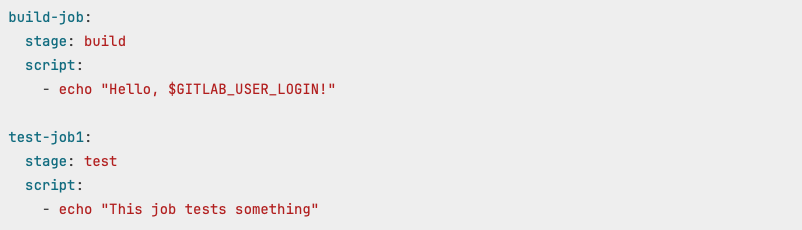
\includegraphics[width=10cm]{resources/ciyaml2.png}
\begin{TUMCodeBlock}{.gitlab-ci.yml}{markdown}
# image of an OS
image: ubuntu:20.04

pytest:
  stage: test
  before_script:
    # update ubuntu
    - apt-get update
    # install pip
    - apt-get install -y python3-pip
    # install python packages
    - pip3 install pytest pytest-cov
  script:
    # run pytest
    - pytest --cov --cov-report term
\end{TUMCodeBlock}
            
            
\end{frame}


\end{document}
